\chapter{Results} \label{ch:results}

\section{Entropy maps}

Looking back at the analysis of the Gray-Scott system by Pearson, in particular \refFig{fig:fk_pspace}, the least stable regions of $F, k$ occur near the bifurcation lines\rf{pearson_1993}. We would expect that patterns with $F, k$ in this region will be the most complex and therefore have higher entropy. In order to elucidate information about the dynamics of the Gray-Scott system, the Shannon entropy \refeq{eq:shannon} is calculated for all $\{ F, k \, | \, F \in [0.004, 0.08], \, k \in [0.03, 0.07] \}$ in an evenly spaced $20 \times 20$ grid (with spacing $dF = 0.004$ and $dk \approx 0.002$) corresponding to the domain of Pearson's map of $F, k$ parameter space (\refFig{fig:fk_pspace}). The diffusion coefficients are fixed at $d_u = 0.16$ and $d_v = 0.08$ for all points. There are then 400 initial values of $F,k$ for which the entropy $S$ is calculated.

In order to increase the resolution of the entropy map, an adaptive resampling method is implemented in the following manner. For any $F, k$ pair of the original 400 points with $S > 0.5$, the entropy is calculated for the four adjacent points $(F \pm dF/2, k)$ and $(F, k \pm dk/2)$ to form a 5 point stencil around the point. This of course requires starting from the Gray-Scott simulation outlined in \refsect{ch1:gs-simulation} and performing the homology calculations for each new $F,k$ pair.

The results of the entropy calculation agree well with our expectations. The plot in \refFig{fig:V144_fk_rs_entropy} shows the entropy $S$ of the Gray-Scott system for chemical $V$ as $F, k$ is varied. Note that systems of higher $S$, the lighter regions of the plot, occur more densely near the dotted line which indicates the Hopf bifurcation. \refFig{fig:UV_entropy} shows the entropy $S$ over the same domain for chemicals $V$ and $U$, respectively, without adaptive sampling (only the initial 400 grid points). These too agree with Pearson's analysis and show that chemicals $U$ and $V$ exhibit similar dynamics.

With 2,500 time steps for each $F,k$, producing a map of the entropy over $F,k$ space requires over 1 million calls to \texttt{chomp-cubical}.\footnote{Computing the Betti numbers of the system is by far the slowest operation and significantly bottlenecks the processing time.} Computed with eight parallel processes on a 4.2GHz Intel i7 processor, this takes about 3-4 days of computation time.

\begin{figure}
	\centering
	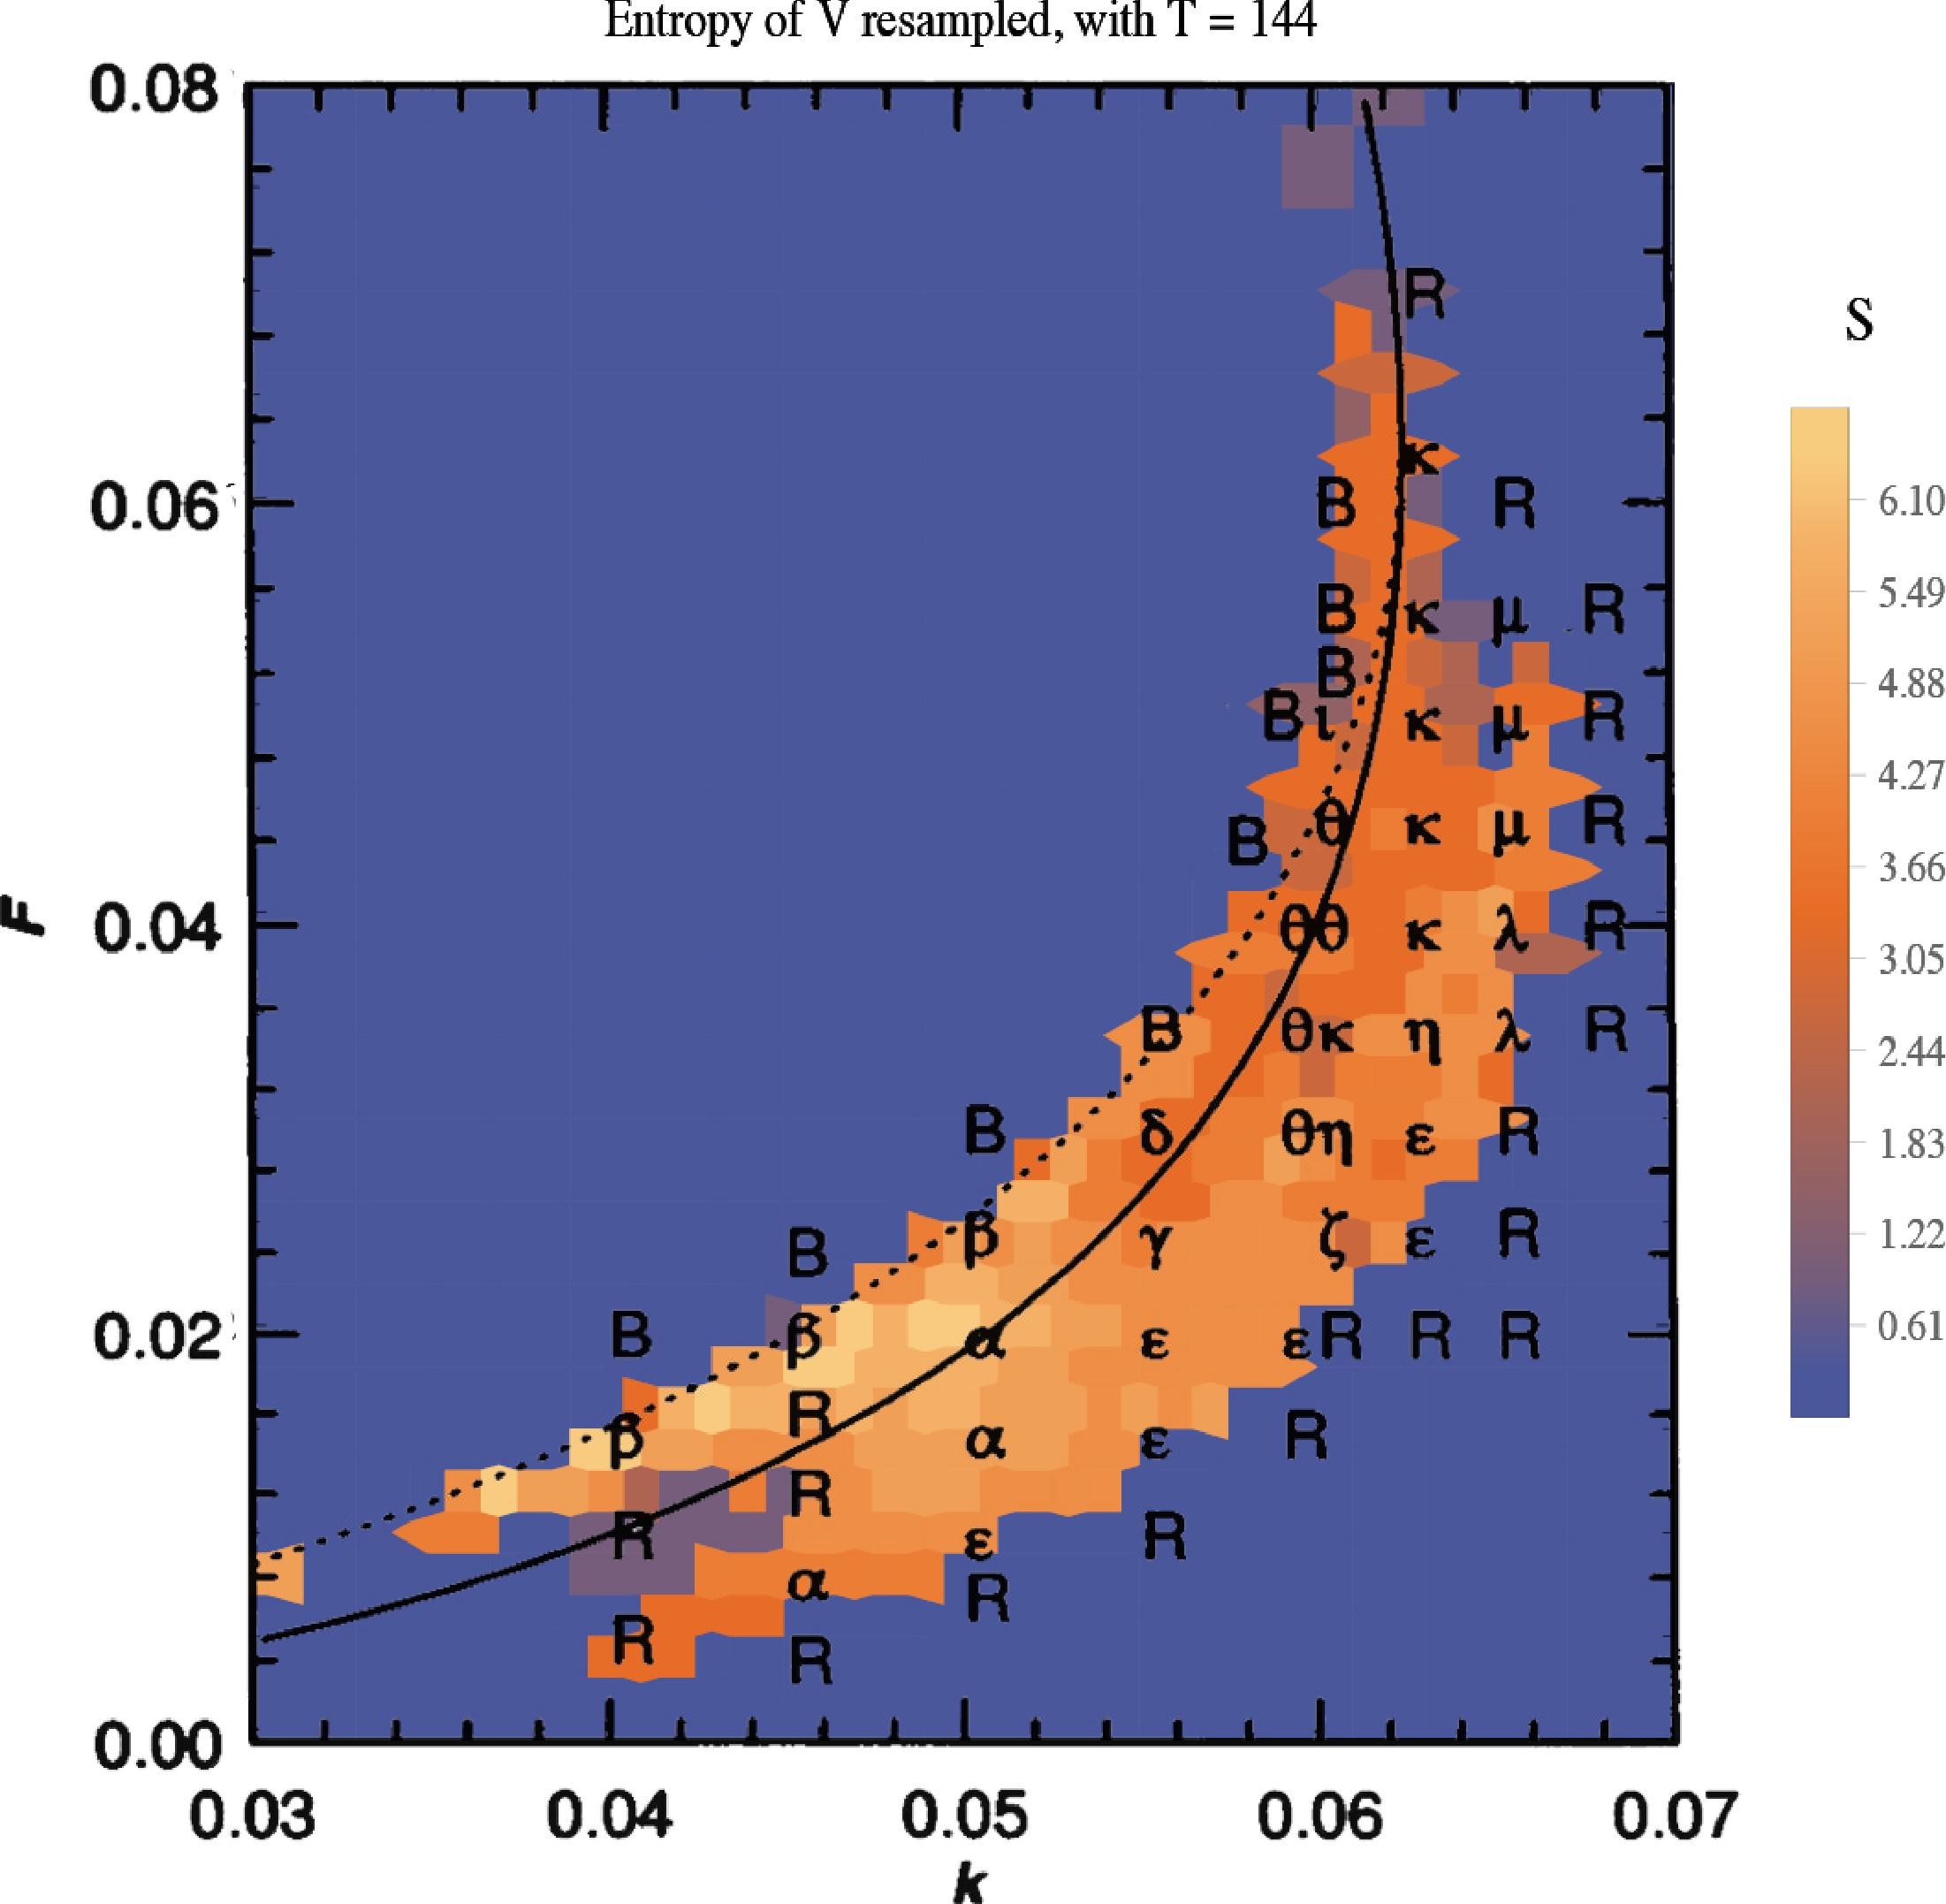
\includegraphics[width=0.7\textwidth]{V144_fk_rs_entropy}
	\caption{A plot of entropy $S$ for the systems described by discrete values of $F, k$ for chemical $V$ with $T = 144$. Adaptive resampling is implemented to increase the resolution of the plot beyond the initial 400 grid points. The phase diagram in \refFig{fig:fk_pspace} is superimposed on the map to illustrate its agreement with Pearson's analysis. The system has higher entropy for $F,k$ values in regions that Pearson identifies as least stable (near the bifurcation lines)\rf{pearson_1993}.} \label{fig:V144_fk_rs_entropy}
\end{figure}

\begin{figure}[hp!]
	\centering
	\begin{subfigure}[b]{0.48\textwidth}
		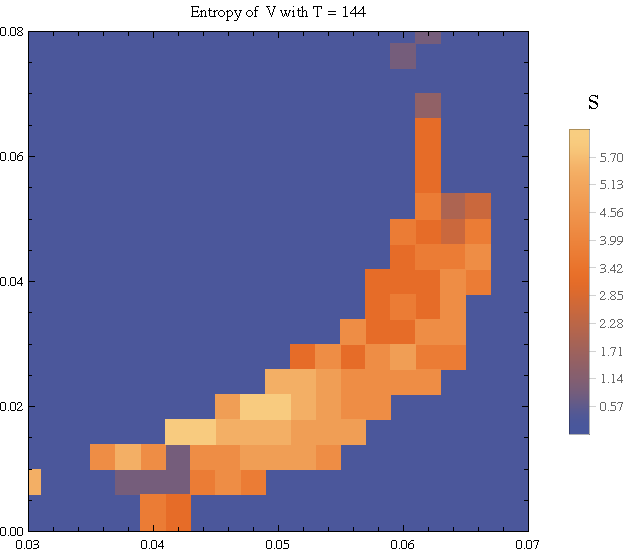
\includegraphics[width=\textwidth]{V144_entropy}
		\caption{Chemical $V$ with $T = 144$.} \label{fig:V144_entropy}
	\end{subfigure} \quad
	\begin{subfigure}[b]{0.48\textwidth}
		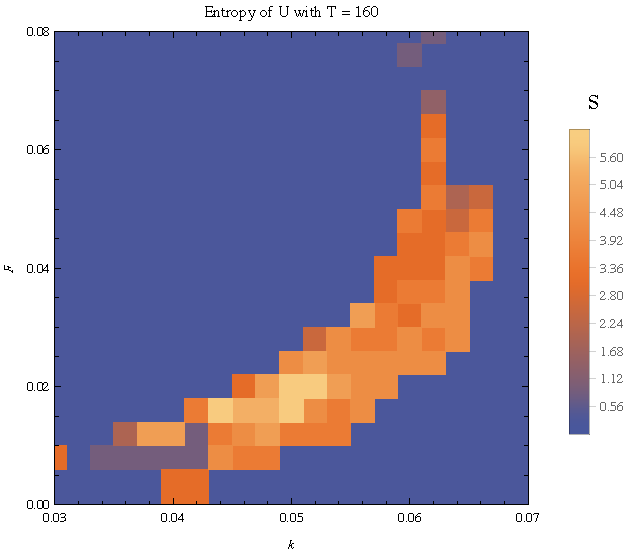
\includegraphics[width=\textwidth]{U160_entropy}
		\caption{Chemical $U$ with $T = 160$.} 
		\label{fig:U160_entropy}
	\end{subfigure}
	\caption{A plot of entropy $S$ for the systems described by discrete values of $F, k$ using only the initial 400 grid points; (a) and (b) show the entropy map for chemicals $V$ and $U$ respectively. Without resampling, the results still agree well with Pearson's analysis; the system has higher entropy near bifurcations where it is least stable. Furthermore, the entropy maps for each chemical species show near perfect agreement.} \label{fig:UV_entropy}
\end{figure}
%
\begin{figure}[p!]
	\centering
	\begin{subfigure}[b]{0.48\textwidth}
		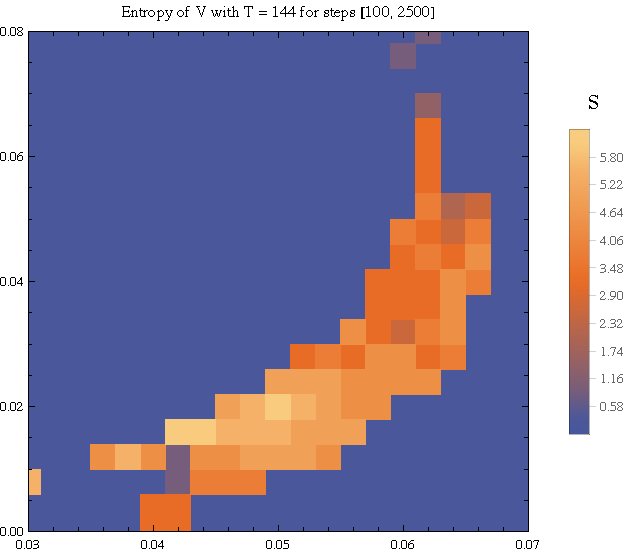
\includegraphics[width=\textwidth]{V144_entropy_trans}
		\caption{Chemical $V$ with $T = 144$} \label{fig:V144_entropy_trans}
	\end{subfigure} \quad
	\begin{subfigure}[b]{0.48\textwidth}
		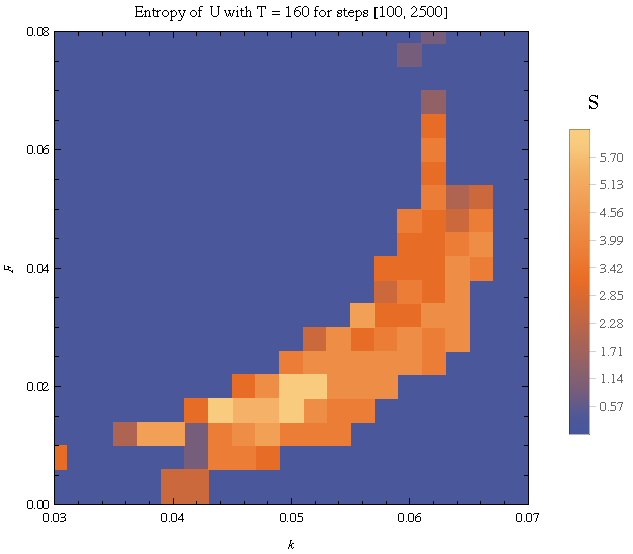
\includegraphics[width=\textwidth]{U160_entropy_trans}
		\caption{Chemical $U$ with $T = 160$} \label{fig:U160_entropy_trans}
	\end{subfigure}
	\caption{A plot of $S$ over $F, k$ space for both chemical $V$ (a) and $U$ (b) considering only time steps $[100, 2500]$ to remove the possible effects of initial transient states. The entropy for each chemical is slightly higher than that shown in \refFig{fig:UV_entropy} where the initial 100 time steps are considered in the entropy calculation.} \label{fig:UV_entropy_trans}
\end{figure}

\section{Transient states}

One consideration in these calculations is the existence of initial transient states. As the Gray-Scott simulation runs, there are about 100 time steps in which the system has not yet reached its steady-state. \refFig{fig:gamma_transients} shows the pattern $\gamma$ at time steps 10, 50, and 100. The time series in \refFig{fig:bplots_gamma} shows how the Betti numbers change as $\gamma$ transitions to the steady-state pattern. Since these initial transient states are not characteristic of the dynamics of the pattern, we may wish to exclude these states in our analysis. The entropy maps in \refFig{fig:UV_entropy_trans} consider only the time steps [100, 2500], ignoring the initial transient states that might affect the calculation of $S$. We see that, in general, $S$ is higher when the transient states are not considered. This makes sense due to the fact that there are not only fewer states to begin with but because the system is not likely to repeat a transient state. In other words, $P_i$ is very low for $i \in [0, 100]$ and the reduction in $N$ (a lower $N$ in \refeq{eq:Pi}) serves only to increase $S$. Either way, the calculation of $S$ is not dramatically affected by removing the transient states.

\begin{figure}
	\centering
	\begin{subfigure}[b]{0.3\textwidth}
		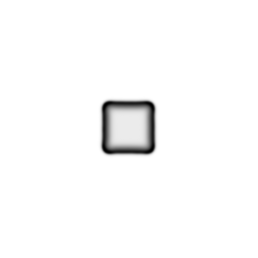
\includegraphics[width=\textwidth]{gamma-0010.png}
		\caption{$\gamma$ at $t_{10}$.} \label{fig:gamma-0010}
	\end{subfigure} \quad
	\begin{subfigure}[b]{0.3\textwidth}
		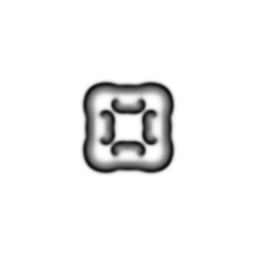
\includegraphics[width=\textwidth]{gamma-0050.png}
		\caption{$\gamma$ at $t_{50}$.} \label{fig:gamma-0050}
	\end{subfigure} \quad
	\begin{subfigure}[b]{0.3\textwidth}
		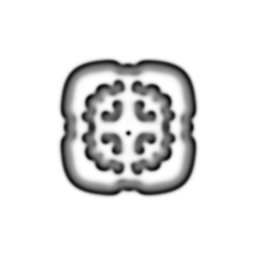
\includegraphics[width=\textwidth]{gamma-0100.png}
		\caption{$\gamma$ at $t_{100}$.} \label{fig:gamma-0100}
	\end{subfigure}
	\caption{Pattern $\gamma$ for time steps $t_{10}$, $t_{50}$, and $t_{100}$. Initial time steps are transient. By time step $t_{100}$, we begin to see features of the steady state pattern.}
	\label{fig:gamma_transients}
\end{figure}

\section{Domain size}

The domain size of the simulation can have a great effect on the entropy of the system. To illustrate this, simulations of patterns $\gamma$, $\epsilon$, $\beta$, and $\delta$ are run with domain sizes $n = 256,\, 512,\, \text{and } 1024$, the results of which are shown in \refFig{fig:domainsize}. We see that the entropy always increases with $n$. This is simply due to the fact that there is more space which greatly increases the complexity of the pattern. The entropy grows faster for some patterns as $n$ increases; pattern $\delta$ shows the greatest rate of change relative to the other patterns. The entropy of the other patterns grows at a consistent rate. \refFig{fig:gamma_domain} illustrates how varying the domain size affects the observed pattern. It is important to note that although the domain size is larger, the underlying dynamics of the system remain unchanged\rf{pearson_1993}.
%
\begin{figure}[h]
	\centering
	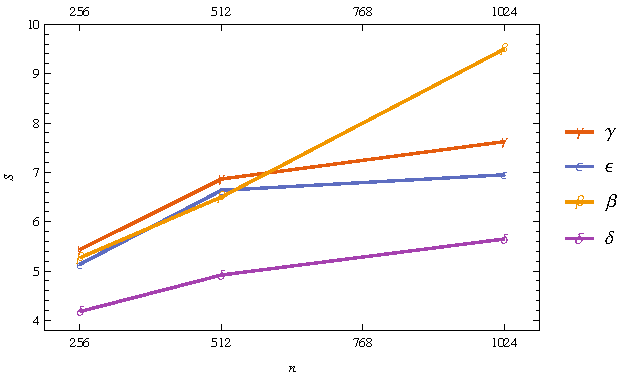
\includegraphics[width=0.8\textwidth]{domainsize}
	\caption{Entropy $S$ of patterns $\gamma$, $\epsilon$, $\beta$, and $\delta$ as the domain size $n$ is increased. Intuitively, the entropy increases with the domain size since there is more space and therefore greater complexity. We notice that $S$ grows faster for some patterns as $n$ is scaled. \refFig{fig:gamma_domain} shows pattern $\gamma$ at the 2000th time step for each domain size $n$.}
	\label{fig:domainsize}
\end{figure}

%\begin{table}[h]
%	\caption{Entropy $S$ of pattern $\gamma$ as the domain size $n$ is varied. Intuitively, the entropy increases with the domain size since there is more space. \refFig{fig:gamma_domain} shows pattern $\gamma$ at the 2000th time step for each domain size $n$.} \label{tab:gamma_domain}
%	\centering
%	\renewcommand{\arraystretch}{1.5}
%	\begin{tabular}{l | l l l }
%	$n$				& 256			& 512			& 1024 \\
%	\hline
%	$S_{\gamma}$		& 5.43427630		& 6.86556517		& 7.62290244 \\
%	$S_{\epsilon}$		& 5.13853135		& 6.63625693		& ?		\\
%	$S_{\beta}$		& 5.27040800		& ?				& ?
%	\end{tabular}
%\end{table}%
%
\begin{figure}[h]
	\centering
	\begin{subfigure}[b]{0.3\textwidth}
		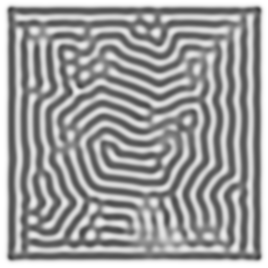
\includegraphics[width=\textwidth]{gamma256-2000.png}
		\caption{$n = 256$} \label{fig:gamma256-1000}
	\end{subfigure} \quad
	\begin{subfigure}[b]{0.3\textwidth}
		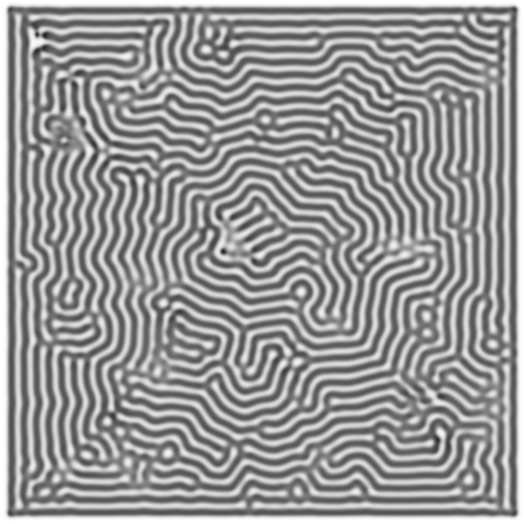
\includegraphics[width=\textwidth]{gamma512-2000.png}
		\caption{$n = 512$} \label{fig:gamma512-1000}
	\end{subfigure} \quad
	\begin{subfigure}[b]{0.3\textwidth}
		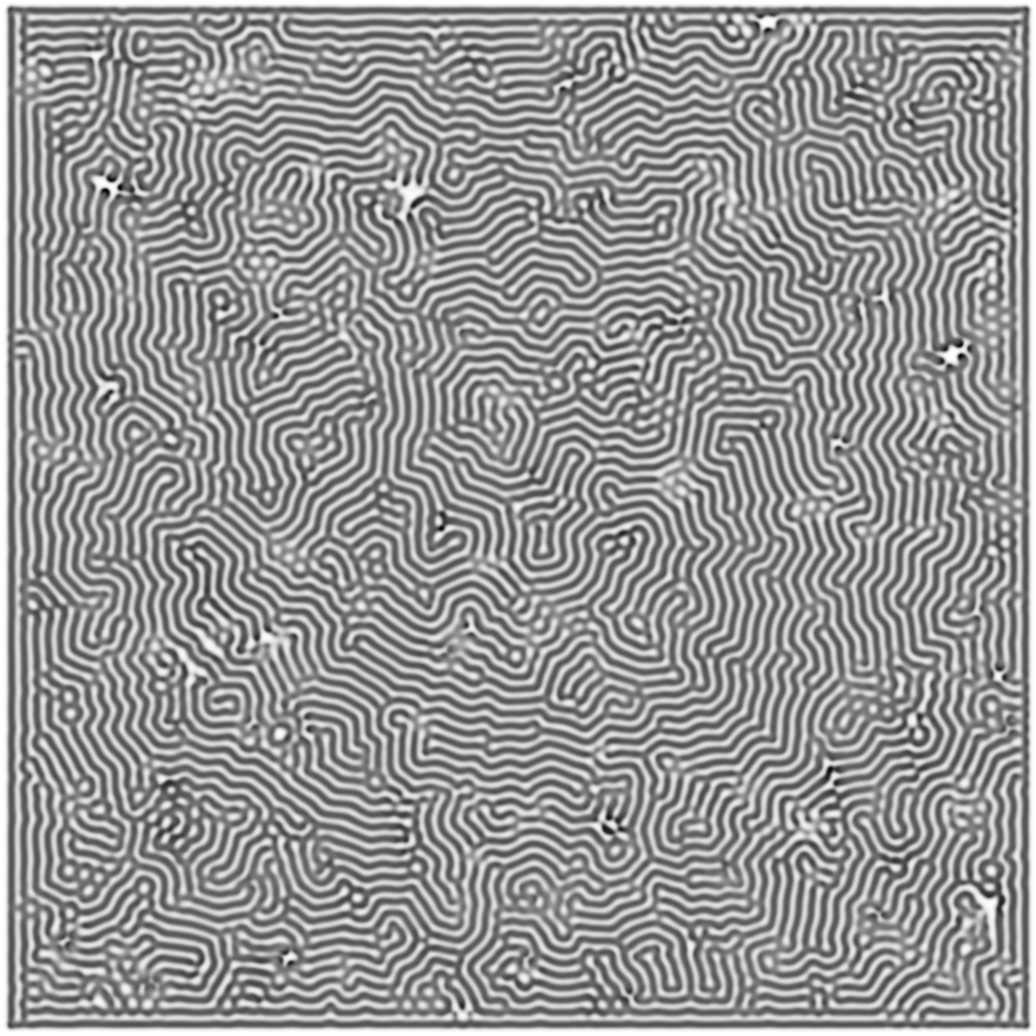
\includegraphics[width=\textwidth]{gamma1024-2000.png}
		\caption{$n = 1024$} \label{fig:gamma1024-1000}
	\end{subfigure}
	\caption{The pattern $\gamma$ at the 2000th time step as the domain size is varied. The spatial complexity increases greatly as $n$ is grows. A plot of the entropy $S$ for each $n = 256,\, 512,\, 1024$ is given in \refFig{fig:domainsize}.} \label{fig:gamma_domain}
\end{figure}

\section{Other systems}

One of the virtues of computational homology is its flexibility in analyzing images. To showcase this, we can examine the homology of a YouTube video. \refFig{fig:smoothlife} shows three frames from a YouTube video of a simulation of the SmoothLife automaton,\footnote{As of this writing, the video is available at \url{https://youtu.be/KJe9H6qS82I}.} a continuous spatial generalization of Conway's ``Game of Life''\rf{smoothlife}. By extracting frames from the video in the form of PNG files and thresholding at $T = 128$, we can calculate the time series of Betti numbers and from there compute the entropy. We use $N$ to indicate the total number of time steps after choosing every $dt$ frames. There are a total of 5400 frames in the video, so the frame step size $dt = 4$, for example, gives $N = 1351$ time steps when considering the entire 3m36s video length. \refTab{tab:smoothlife} gives the entropy $S$ for $dt = 3$, $dt = 4$, and $dt = 5$. The entropy is highest for $dt = 3$, $S = 6.82$, which is also greater than any $S$ in the Gray-Scott entropy map in \refFig{fig:V144_fk_rs_entropy}. This is unsurprising since the SmoothLife simulation video is extremely dynamic.
%
\begin{table}
	\caption{The entropy $S$ of the SmoothLife simulation video for different step sizes and number of time steps.} \label{tab:smoothlife}
	\centering
	\renewcommand{\arraystretch}{1.5}
	\begin{tabular}{l | l l l }
	$dt$, $N$		& 3, 1800		& 4, 1351		& 5, 1081 \\
	\hline
	S			& 6.82	& 6.67		& 6.54
	\end{tabular}
\end{table}%

\begin{figure}[h]
	\centering
	\begin{subfigure}[b]{0.3\textwidth}
		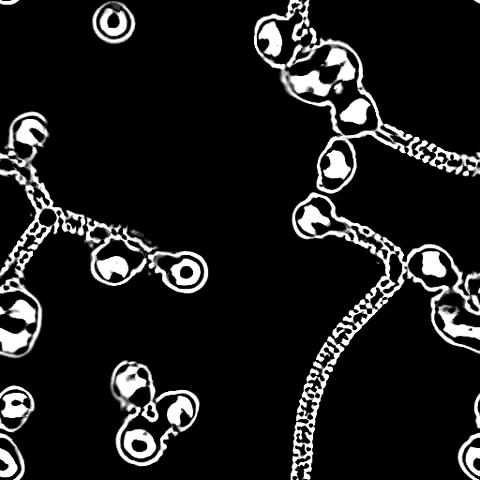
\includegraphics[width=\textwidth]{sl02421.png}
		\caption{$\beta_0 = 52$, $\beta_1 = 40$} \label{fig:sl2421}
	\end{subfigure} \quad
	\begin{subfigure}[b]{0.3\textwidth}
		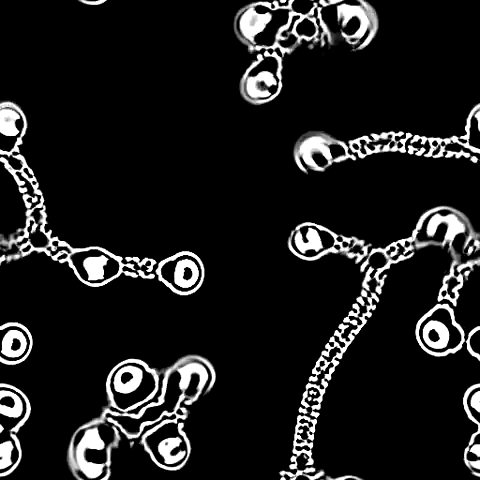
\includegraphics[width=\textwidth]{sl02436.png}
		\caption{$\beta_0 = 67$, $\beta_1 = 41$} \label{fig:sl02436}
	\end{subfigure} \quad
	\begin{subfigure}[b]{0.3\textwidth}
		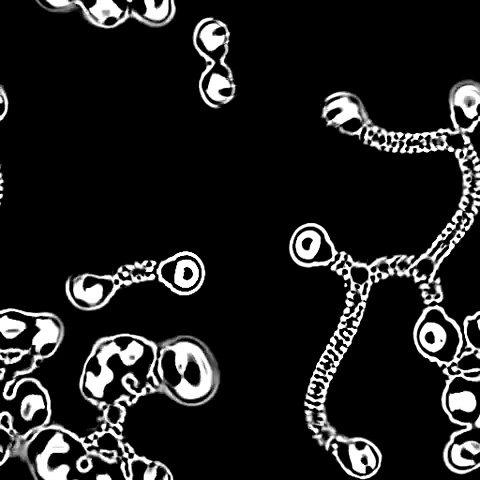
\includegraphics[width=\textwidth]{sl02451.png}
		\caption{$\beta_0 = 78$, $\beta_1 = 43$} \label{fig:sl02451}
	\end{subfigure}
	\caption{Three near-consecutive frames from a video of a SmoothLife simulation (before thresholding). The Betti numbers $\beta_0, \beta_1$ are given for reference. In this case, $\beta_0$ and $\beta_1$ consider white and black respectively. Computing the Betti numbers of every 3 frames gives $S = 6.82150758771$ which is highly entropic. Images adapted from \protect\bibentry{smoothlife}.} \label{fig:smoothlife}
\end{figure}